\section{B{\'e}zier curves and \acs{NURBS}}
\label{sec:NURBS}

\tododone[inline]{Erik: expand this! and a better name}
\tododone[inline]{Erik: split this section into two: fitting and NURBS}

\emph{\Bez curves} and \emph{\acl{NURBS}} (\acs{NURBS}) are two types of curves which are very important in CAD (see \autoref{sec:CADbackg} above) used mainly to model surfaces. They are both defined parametrically by creating linear combinations of a set of \emph{control points}, with the coefficients in these linear combinations being functions of the input parameter. There are many reasons behind their popularity, some of them being their relatively straightforward way of calculation and approximation, and the intuitive way of modification by changing the control points. In this section, we will provide definitions and backgrounds on them, as well as a description of \emph{Peters' scheme}, a scheme for constructing a smooth ($G^1$) surface from the vertices in a polygonal mesh. For a  more in-depth introduction and further material about NURBS, we refer to \cite{farin2002handbook}, and for further reading about Peters' scheme, we refer to the original article \cite{peters1992constructing}.

%Parametrised geometries are often given in terms of \emph{Non-Uniform Rational B-Spline} (NURBS) curve patches (see for example the documentation of the CAD software FreeCAD in \cite{FreeCAD}). 
%In this section we will discuss:
%\begin{itemize}
%\item Parametrized curves and surfaces such as Bezier and NURBS surfaces
%\item Peters' Scheme, a scheme for generating tangent plane continous ($G^1$) surfaces from an unstructured mesh of polygonal faces as first described in...[ref]
%\item Possibly how to fit this surface to parametrized datapoints using least squares. That could be impl.
%\end{itemize}


\subsection{Parametric Curves}
\label{subsec:paracurves}
To define NURBS from a mathematical standpoint, we first define so-called \emph{\Bez curves} and use them later for the definition of NURBS. 
\subsubsection{\Bez Curves}
\label{subsub:bezcurvsurf}
A \Bez curve is a \textit{parametric} curve, which is often used for producing a smooth approximation of a given set of data points.
 
An analytical expression for the \Bez curve parametrized by the variable $u$ is given by:
\begin{equation}
\label{eq:beziercurve}
\vec{B}(u)=\sum\limits_{i=0}^n b_i^n(u) \vec{p}_i
\end{equation}
where $\vec{p}_i$ is the $i^{\text{th}}$ control point, $i\in0,1, \dots ,n$ ($n+1$ control points in total), and
\begin{equation*}
b_i^n(u)=\binom{n}{i}(1-u)^{(n-i)}u^i
\end{equation*}
with $\binom{n}{i}$ being a binomial coefficient, is the $i^{\text{th}}$ \emph{Bernstein polynomial} (see \cite{lorentz2012bernstein}) of degree $n$.

In addition to the expression with Bernstein polynomials, one can use a recursion formula (so-called \emph{de Casteljau Algorithm}) for the construction of the \Bez curve, which we will not cover here. 

Analogous to \Bez curves, one can also define a \textit{\Bez surface}. One way of doing this is by extending the set of control points indexed in one dimension, to a two-dimensional mesh of $n\times m$ control points $\vec{p}_{i,j}$. Likewise, we extend the Bernstein polynomial basis to $2$D by taking its tensor product with itself. The resulting \textit{tensor product \Bez surface} is then given by the analytical expression
\begin{equation}
\label{eq:bezsurface}
\vec{S}(u,v)=\sum\limits_{i=0}^n \sum\limits_{j=0}^m b_i^n(u) b_j^m(v) \vec{p}_{i,j}
\end{equation}

\subsubsection{B-Splines and NURBS}
Extending the idea described in previous section, one could use \emph{B-spline basis functions} (see below) instead of the Bernstein polynomial basis.

Unlike \Bez curves, the parameter domain for B-splines is subdivided by so-called \textit{knots}. For the one-dimensional parameter domain $[u_{0}, u_{m}]$, the \textit{knot vector} will be given by $u_{0} \leq u_{1} \leq ... \leq u_{m}$. In most cases $u_{0} = 0, u_{m} = 1$ is chosen, so that we get a unit interval for our parameter values. For the case of NURBS, the knots $u_{0},..., u_{m}$ need not be equidistant -- hence the "NU" (for Non-Uniform) in the name "NURBS".

Given a knot vector $[u_{0}, u_{m}]$ and a degree of B-spline $p$, the $i$-th B-spline basis function is then defined recursively as follows:
\begin{equation}
N_{i,0}(u) =  \begin{cases} 1, & \mbox{if } u_{i} \leq u < u_{i+1} \\ 0, & \mbox{otherwise } \end{cases}
\end{equation} 
\begin{equation}
N_{i}^p(u) = \frac{u - u_{i}}{u_{i+p} - u_{i}}N_{i}^{p-1}(u)  + \frac{u_{i+p+1}-u}{u_{i+p+1} - u_{i+1}}N_{i+1}^{p-1}(u)
\end{equation}
For $p=0$ the basis fucntions are simply step functions, and for $p=1$ we end up with so-called "hat" functions. Quadratic basis functions ($p=2$) look more complicated (\autoref{fig:bsplineBases}).
\begin{figure}
\centering
\begin{subfigure}[b]{.3\linewidth}
  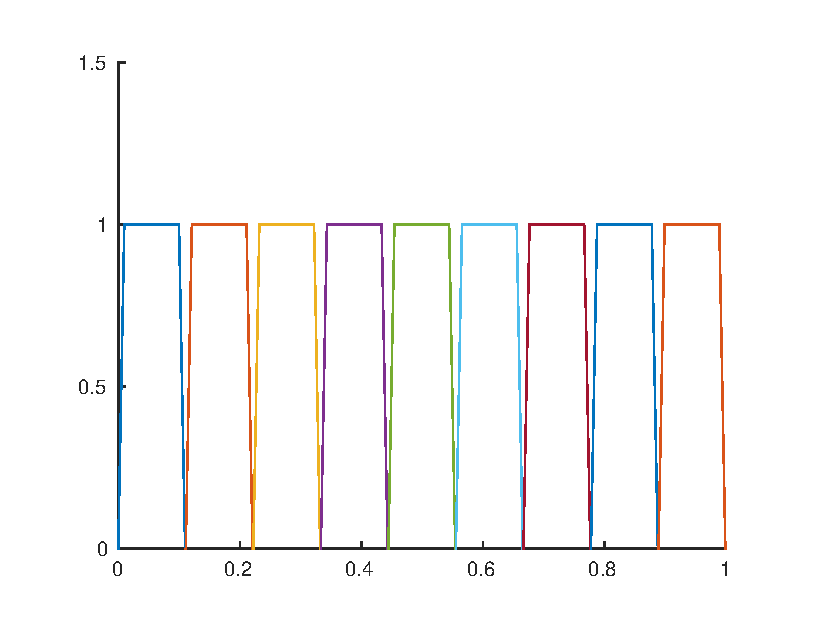
\includegraphics[width=\linewidth]{Pictures/basisconstant}
  \subcaption{B-spline basis for $p=0$}
  \label{fig:bspline_basis_constant}
\end{subfigure}%
\begin{subfigure}[b]{.3\linewidth}
  \includegraphics[width=\linewidth]{Pictures/basislinear}
  \subcaption{B-spline basis for $p=1$}
  \label{fig:bspline_basis_linear}
\end{subfigure}
\begin{subfigure}[b]{.3\linewidth}
  \includegraphics[width=\linewidth]{Pictures/basisquadratic}
  \subcaption{B-spline basis for $p=2$}
  \label{fig:lognorm_quadratic}
\end{subfigure}
\caption{B-spline basis functions, of degree $p=0$ (left), $p=1$ (middle) and $p=2$ (right).}
\label{fig:bsplineBases}
\end{figure}


By giving each of these basis functions a weight $\omega_i$ and normalizing them at each point by dividing by the total sum, we get the rational basis functions. Writing them out explicitly, in terms of B-spline basis functions $N_{i,p}$, the $n^{\text{th}}$-degree NURBS surface with $k$ control points $P_i$ is finally given by:
\begin{equation}
\label{eq:nurbscurve}
\vec{C}(u) = \frac{\sum_{i=1}^{k}N_i^n\left(u\right)\omega_{i}\vec{p}_{i}}{\sum_{i=1}^{k}N_i^n\omega_{i}}.
\end{equation}

B-splines have the following properties, which are useful for our problem:
\begin{itemize}
\item Degree $n$ and number of control points $\vec{P}_{i\cdots m}$ are independent.
\item B-Splines only change locally (depending on the degree $n$) when a control point is changed.
\end{itemize}

Analogous to the tensor product \Bez curve surfaces (see \autoref{eq:bezsurface}), one can define tensor product B-spline or NURBS surfaces:
\begin{equation}
\label{eq:nurbssurface}
\vec{S_\text{NURBS}}(u,v)=\frac{\sum\limits_{i=0}^n \sum\limits_{j=0}^m N_{i}^n(u) N_{j}^m(v) \omega_{i,j}\vec{p}_{i,j}}{\sum\limits_{i=0}^n \sum\limits_{j=0}^m N_{i}^n(u) N_{j}^m(v) \omega_{i,j}},
\end{equation}
where the case with all $\omega_{i,j} = 1$ corresponds to a B-Spline surface; respectively a NURBS surface if any $\omega_{i,j} \neq 1 $. With varying degrees and number of control points, these can be made to fit a variety of shapes. However, as the parameters $u$ and $v$ define a square in their two-dimensional parameter domain, there is a limit to what topologies may be realized with just one such NURBS surface. For example, an open cylinder could be constructed by one such surface where one of the sides meets its own beginning, whereas something with multiple holes - like a double torus, or a non-flat 8-shaped surface, would be impossible. Therefore, when using NURBS, surfaces are most often modelled using a network of connected patches. \todointern{maybe should include an example picture here} For more information about NURBS, see \cite{farin1999nurbs}.

\subsection{Peter's Scheme}
\todo[inline]{insert stuff here}
In this section we will cover the following, reffering to paper[]:
\begin{itemize}
\item How we go from polygonal faces to a set of mesh control points. "patch points", specifying that we're talking about quads, and that we then get 16
\item That for each of these 16 points, we will make a small Bezier patch
\item That if we define the Bezier control points of these patches in a special way, as described in appendix XYZ \todo{TODO: create this appendix, or change this to refer to paper for coefficients}, we get a surface that is $G^1$ continous
\item Maybe describe that we then need for every one of these Bezier patches the locations of the neighbours
\item That the location of a point on the surface defined by parameters $\vec{s} = (u,v)$ depends on the Bezier control points, whose linear dependence on the "patch points" give us coefficients on these "patch points" of the location described by the parameters, as can be seen in \autoref{fig:PetersPoints}
\item Possibly that this can used to fit the location of these "patch points" to a set of datapoints by minimusing a least-squares error 
\end{itemize}
\begin{figure}

\missingfigure{Graphical descirption of all those different points in peter's scheme}
\label{fig:PetersPoints}
\caption{The points in Peter's scheme. As clearly seen in the figure above, this scheme is self-explanatory.}
\end{figure}